\usetikzlibrary{arrows.meta,calc}
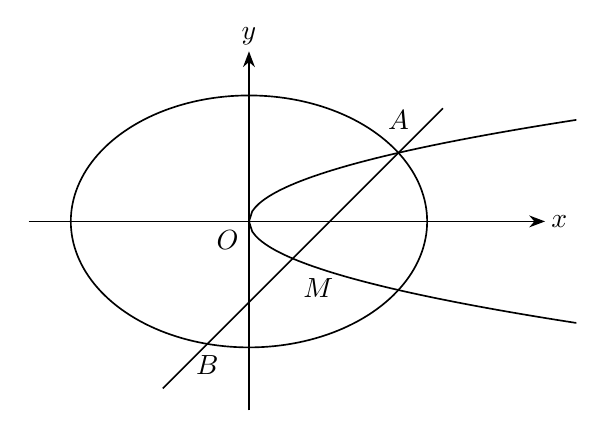
\begin{tikzpicture}[x=1.6cm,y=1.6cm,line width=.6pt,font=\normalsize,>=Stealth]
\def\ellA{1.4142136}
\def\ellB{1}
\def\parp{0.125}
\coordinate (O) at (0,0);
\coordinate (A) at (1.1861407,0.5445504);
\coordinate (B) at (-0.3306870,-0.9722772);
\coordinate (M) at (0.3470398,-0.2945504);
\coordinate (La) at (1.5397,0.8982);
\coordinate (Lb) at (-0.6843,-1.3259);
\draw[->] (-1.75,0)--(2.35,0) node[right,inner sep=0pt,xshift=2pt] {$x$};
\draw[->] (0,-1.5)--(0,1.35) node[above,inner sep=0pt,yshift=2pt] {$y$};
\draw plot[domain=0:360,samples=181,variable=\t] ({\ellA*cos(\t)},{\ellB*sin(\t)});
\draw plot[domain=0:2.6,samples=101,variable=\t] ({\t},{sqrt(2*\parp*\t)});
\draw plot[domain=0:2.6,samples=101,variable=\t] ({\t},{-sqrt(2*\parp*\t)});
\draw (Lb)--(La);
\node[above=7pt,inner sep=1pt] at (A) {$A$};
\node[anchor=north,inner sep=0pt,yshift=-4pt] at (B) {$B$};
\node[anchor=center,inner sep=0pt] at (0.55,-0.53) {$M$};
\node[anchor=center,inner sep=0pt] at (-0.17,-0.15) {$O$};
\end{tikzpicture}
